\documentclass[12pt]{article}

% Displaying maths
\usepackage{amsmath}
\usepackage{amssymb}

% Displaying figures
\usepackage{graphicx} 	% include graphics with the command \includegraphics
\usepackage{rotating} 	% for sideways tables

% Double spacing
%\usepackage{setspace} 
%\doublespacing

% Page layout
\topmargin 0.0cm
\oddsidemargin 0.5cm
\evensidemargin 0.5cm
\textwidth 16cm 
\textheight 21cm

% Bold the 'Figure #' in the caption 
\usepackage[labelfont=bf,labelsep=period,justification=raggedright]{caption}

% Bibliography package natbib
\usepackage[round]{natbib}

% Title page
\title{PhD Literature Review MS}
\date{}
\author{}


%%%%%%%%%%%%%%%%%%%%%%%%%%%%%%%%%%%%%%%%%%%%%%%%%%%%%%%%%%%%%%%%%%%%%%%%%%%%%%%%%%%%%
%%%%%%%%% 		PhD Literature Review			%%%%%%%%%%%%%%%%%%%%%
%%%%%%%%% 		Draft 5 				%%%%%%%%%%%%%%%%%%%%%
%%%%%%%%% 		Magnus Clarke 				%%%%%%%%%%%%%%%%%%%%%
%%%%%%%%% 		20.11.13 				%%%%%%%%%%%%%%%%%%%%%
%%%%%%%%%%%%%%%%%%%%%%%%%%%%%%%%%%%%%%%%%%%%%%%%%%%%%%%%%%%%%%%%%%%%%%%%%%%%%%%%%%%%%


\begin{document}
\maketitle
\tableofcontents
\newpage

\section{Introduction}

Evolution is heritable change through time. Over long timescales, the discrete objects subject to change are species. Phylogenies are trees showing species, speciation events and their arrangement in time. Since the advent of evolutionary theory, species have been compared with each other to suggest adaptive explanations for their trait values. Similar trait values, however, can also be due to shared ancestry; hence, we infer jointly the phylogenetic and ecological effects on trait values. This is aided by the wealth of reliable phylogeny data now obtainable from DNA sequencing.

To infer evolutionary processes from trait data, we require models of these processes that predict trait data. These models have two forms: they can predict trait evolution along a branch of a phylogeny, or they can predict the times at which branches will bifurcate. 

The evolutionary models are outlined here, along with models which associate discrete amounts of evolutionary change with speciation events. The biological expectations and evidence for these models are discussed, and future developments are briefly considered.

\section{Models of continuous evolution}

\subsection{Data}

Models of continuous change on a phylogeny rely on three pieces of data:
\begin{itemize}
  \item Tree topology;
  \item Branch lengths;
  \item Trait values of tree tips.
\end{itemize}

These models give instantaneous rates of evolution as a function of position on the phylogeny branch. Then, the difference between two species is predicted from the length of branches separating them. The tendency for phylogenetically close species to be phenotypically similar is referred to as `phylogenetic signal' \citep{blomberg_testing_2003}. Phylogenetic niche conservatism (PNC) is a related concept, with no universal definition \citep{cooper_phylogenetic_2010}. Loosely, it is phylogenetic signal where the trait is the species' niche. Phylogenetic signal is often assumed to be particularly strong for such traits, but this assumption may be frequently unsatisfied \citep{losos_phylogenetic_2008}. 

The best data for comparative analyses consists of many closely related pairs of species that differ in trait value, with each pair well separated phylogenetically from the others \citep{garland_phylogenetic_2005}. Ancestral trait values can be very useful in fixing non-tip phylogeny nodes, but are rare and generally not incorporated into phylogenetic comparative analyses \citep{harmon_early_2010}. 

\subsection{Evolution on branches}

The need to account for phylogeny in comparative analyses was first made clear by \citet{felsenstein_phylogenies_1985}. He used a model where the change in trait value in a short period of time is drawn from a normal distribution: this is Brownian Motion (BM). Other models of trait evolution along a branch are derived from the BM model by adding parameters. Here, the various models are listed in time-differential form in Table 1. 

The BM model has a trait value X evolving at random, at a rate $\sigma$:

\begin{equation}
	dX(t) = \sigma dW(t)
\end{equation}

where W(t) is the integral of the continuous white noise function, such that $ \Delta W_t \sim N(0, ~\Delta t)$. If used to predict trait values at a time T, the BM model has two free parameters: the evolutionary rate $\sigma$ and the root trait value X(0).

The parameter $\lambda$ \citep{pagel_inferring_1997,pagel_inferring_1999} measures the goodness of fit of trait data to those expected under a given BM model.  A value of 1 indicates a perfect fit to the BM model; $\lambda<1$ indicates less phylogenetic signal and $\lambda>1$ indicates more signal than expected. 
$\lambda$ can be represented as a transformation of the tree into one with internal branches scaled by the factor $\lambda$.

We know that rates of evolution vary. How do we add plausible patterns of rate-change to the BM model? Looking at equation 1, we seem to have two options: we can elevate the factor $\sigma$ to the status of a function, or we can add a separate, deterministic term to the equation. Time-dependency of $\sigma$ could be linear ($ \sigma \rightarrow (t_{max}-t)\sigma$), polynomial ($ \sigma \rightarrow  \kappa t^{\kappa - 1} \sigma $), or exponential ($ \sigma  \rightarrow g^{-t} \sigma $). 

\begin{figure}[!ht]
	\begin{center}
	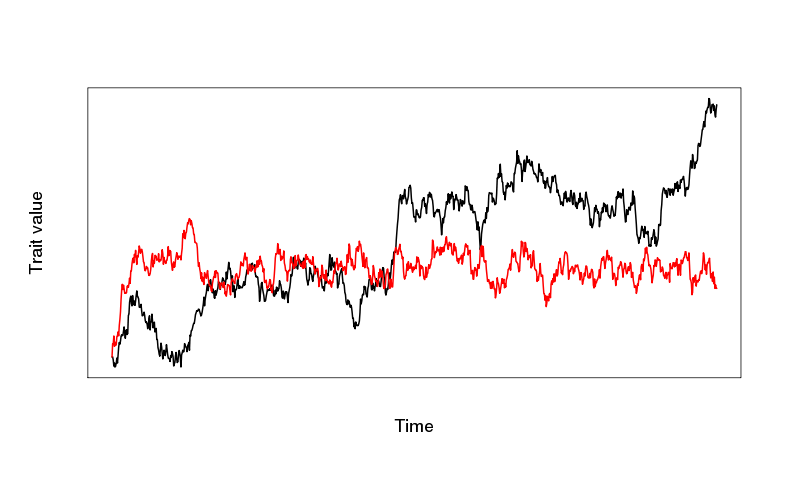
\includegraphics[width=6in]{../figures/sim}
	\end{center}
	\vspace{-40pt}	
	\caption{
		An example of evolution under the BM (black) and OU (red) models.
	}
	\label{Figure_label}
\end{figure}

Polynomial time dependence $\kappa$ is first seen in \cite{pagel_inferring_1997}.
Exponential models, meanwhile, are termed Accelerating/Decelerating (ACDC) models \citep{blomberg_testing_2003}. Each of these models adds one free parameter to the BM model.
One more alternative exists and has been implemented: the evolutionary rate $\sigma$ may be a step function of time; these steps (i.e. discrete rate changes) may represent sudden environmental changes, or transitions into or out of ecological niches \citep{thomas_comparative_2006, o'meara_testing_2006}. If some extrinsic event is known about, then the positions of the corresponding steps can be built into the model before the model is used. Alternatively, maximum likelihood (ML) positions and sizes of discrete rate changes can be estimated from the data \citep{thomas_motmot:_2012,revell_new_2012}. 

The second way to modify the BM model of equation 1 is to add an additional term. In the OU model \citep{hansen_stabilizing_1997} the trait X is drawn towards a central value ('primary optimum') $\psi$ with a strength proportional to its distance from the optimum:

\begin{equation}
	dX(t) = - \alpha (X(t) - \psi) dt + \sigma dW(t)
\end{equation}

\begin{figure}[!ht]
	\begin{center}
	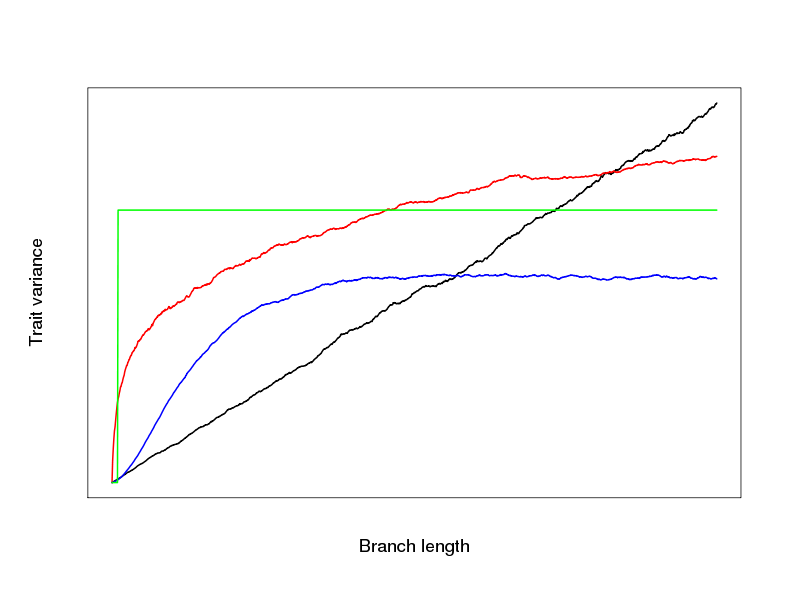
\includegraphics[width=6in]{../figures/var}
	\end{center}
	\vspace{-40pt}	
	\caption{
		Variance among tip trait values under different models of evolution. Branch lengths in units of time. The black line is the BM model; the red line is $\kappa < 1$; the blue line the OU model, with a different optimum for each branch; the green line is a NF model.
	}
	\label{Figure_label}
\end{figure}
\vspace{20pt}

For this reason, the OU model is sometimes called the 'single stationary peak' (SSP) model.
It is perhaps easier to imagine this as an ecological process of avoiding extreme trait values: as a species gets further from the clade mean, it becomes more likely to evolve towards the clade mean. 
(Being repelled by two extreme values is of course equivalent to being attracted to one central value).

The OU model can be extended by adding discrete optima shifts based on prior knowledge of extrinsic events, or with  methods to estimate ML positions of optima shifts \citep{hansen_stabilizing_1997,hansen_assessing_2005}. Additionally, the optima may themselves evolve according to a BM or OU model \cite{hansen_measuring_2008,hansen_interpreting_2012}. 

\subsection{Evolution on phylogenies}

Most of the BM-like models of evolution can be applied separately to each branch, but we can also make evolutionary rates dependent on position in the whole phylogeny. Firstly, we might test for a phylogeny-wide change in the rate of evolution, analogous to the within-branch parameter $\kappa$ \citep{pagel_inferring_1997}. This parameter takes the same form as $\kappa$, and is referred to as $\delta$ \citep{thomas_motmot:_2012} (See Table 1). We can also permit rate parameters to be branch-specific. 
Having an independent $\sigma$ for each branch is possible \citep{mooers_using_1999}, but will tend to lead to too many free parameters \citep{thomas_motmot:_2012}. ML estimation of a limited number of discrete rate changes, however, can be applied clade-wise as well as time-wise, so that a change appears on just one branch in a phylogeny, but is inherited by subsequent `offspring'.

\subsection{Stretching branches}

If phylogeny branch lengths represent time, then the evolutionary models in the previous section allow us to calculate the amount of change per branch - not necessarily proportional to time. The evolutionary models can also be viewed as maps from time-scaled trees into change-scaled trees. The BM model is then the identity operator. Some of the models were originally presented as such a transformation. An example tree transformed under each model is shown in Figure 3.

%LOOK UP LANDIS 2013, VENDITTI ET AL 2011, EASTMAN ET AL 2012

\begin{figure}[!ht]
	\begin{center}
	\includegraphics[width=6in]{../figures/trees}
	\end{center}
	\vspace{-40pt}	
	\caption{
		Change-scaled trees. The BM tree is identical to the time-scaled tree, and different evolutionary models are different transformations into other trees. Kappa and delta are between 0 and 1.
	}
	\label{Figure_label}
\end{figure}
\vspace{20pt}

\subsection{Multiple traits}

The BM and BM-like models generalise immediately to multiple traits: the trait value X becomes a vector of trait values $\overrightarrow{X}$, and the rate parameter $\sigma$ becomes a covariance matrix $\boldsymbol{\Sigma}$. Nonzero nondiagonal elements of $\boldsymbol{\Sigma}$ indicate correlation between traits. 

One of the main uses for phylogenetic methods is to measure correlations between traits while controlling for the phylogeny. This is discussed in Section 4, but it may be useful to note a potential source of confusion: many methods seek to separate phylogenetic and ecological effects. However, ecology may be heritable. If two species are labile but have phylogenetic signal due to shared inherited ecology, then they are independent data points with respect to the details of that ecology, but non-independent with respect to general ecological principles.
 
OU model variants have been developed to account for coadaptation between traits, with trait optima either fixed or evolving by the BM model. With multiple traits, $\alpha$ becomes a matrix, and off-diagonal elements can permit one trait's optimum to change according to another trait's value, even if the second trait is simply evolving according to BM \citep{bartoszek_phylogenetic_2012}.

\section{Models of speciation-based evolution}

\subsection{Evolution on phylogenies}

Branch-evolution parameters such as $\kappa$ can be used as a test for speciational evolution. An alternative is simply to postulate a `lump' of trait change at each speciation event, with the lump drawn from N(0, $\sigma_c$) \citep{bokma_detection_2008, ingram_speciation_2010}. If the speciation rate is $\xi$, then we can measure the degree to which rapid evolution is linked to speciation events with the value of

\begin{equation}
	\frac{\xi \sigma^2_c}{\sigma^2_{total}}   %\in [0,1]
\end{equation}

This model requires extinction rate estimates. Methods to generate extinction rate estimates exist \citep{rabosky_heritability_2009,pybus_testing_2000}, but it is not clear how to get these without first making assumptions about the evolutionary model that we are hoping to test.

If the amount of Brownian Motion is set to zero, then the \cite{ingram_speciation_2010} model reduces to random amounts of trait change at speciation events and none in between speciation events. This corresponds to a pure `punctuated equilibrium' model of evolution.

Niche-filling (NF) models \citep{freckleton_detecting_2006,price_correlated_1997,harvey_comparative_2000} also have purely speciational modes of evolution, but have a few differences from the Ingram model. In niche-filling models, species' trait values are constant in time, and the position of each niche in niche-space is constant in time. New niches are filled by new species, branching from whichever species is closest in niche-space. 
\citet{freckleton_detecting_2006} distinguish between NF models where every species is equally likely to speciate and form a new and filled niche, and NF models where niches appear at a constant rate, randomly positioned in niche-space. The two are equivalent when all the species have evenly distributed trait values, but have different predictions otherwise; for example, a species particularly distant from all others in trait-space will be more likely to speciate under the randomised NF model.

In the Ingram model speciation is a splitting process, where each of the two species shifts to a new trait value. Hence, in NF models speciation is a branching process, where only the `new' species moves to a new trait value. This leads to a difficulty for NF models, however: if a lineage splits and the 'original' lineage subsequently goes extinct, then a phylogeny built from extant species will have unexplained mid-branch evolutionary change (assertion).

A further model combines phylogenetic signal from a BM process with a postulate of trait variance increasing linearly with spatial separation between the species \citep{freckleton_space_2009}. The relative importance of the two terms of the expression for the variance then measures the importance of physical locale in the evolution of the trait.

\begin{sidewaystable}
%\begin{table}[!ht]
\caption{Models and parameters for evolution on a known phylogeny. Multi-trait parameter counts are upper limits assuming free covariance between all traits.}
\begin{tabular}{l l l l}
\hline
Model & Equation & parameters & parameter count 	 \\
\hline
BM              & $dX(t) = \sigma dW(t)$                        & root value, $\sigma$=rate             & 2    		\\ 
		& $var(X) = T \sigma^2$ 			& T is time from common ancestor 	& 		\\
$\kappa$        & $dX(t) = \kappa \sigma t^{\kappa -1} dW(t)$   & $\kappa > 0$, t from branch start     & 3     	\\
		& $var(X) = \Sigma_i T_i \sigma$ 		& i labels each branch, and $T_i$ is its length & 	\\
$\delta$        & $dX(t) = \delta \sigma t^{\delta -1} dW(t)$   & $\delta > 0$, t from tree root        & 3     	\\
		& $var(X) = \sigma^2(T^{\delta} - T_0^{\delta}$ & T is time over tree, $T_0$ is time of MRCA & 		\\ 
Step            & $dX(t) = \sigma(t, clade) dW(t) $             & $\sigma$ step fn with m steps         & 1+2m   	\\
ACDC            & $dX(t) = \sigma g^{-t} dW(t)$                 & $ g > 0 $                             & 3     	\\
OU              & $dX(t) = -\alpha(X(t)-\psi)dt+\sigma dW(t)$    & $\psi$ is optimum, strength $\alpha$  & 4    	\\
		& $var(X) = \frac{\sigma^2}{2\alpha}(1-e^{-2 \alpha T})$ 	& & 					\\
stepOU          & $dX(t) = -\alpha(X(t)-\psi_i)dt+\sigma dW(t)$  & i is number fitted optimum shifts     & 4    	\\
Ingram2010      & BM + $N(0, \sigma^2_c)$ per speciation        &                                       & 3     	\\

\hline
\end{tabular}
\label{tab:label}
%\end{table}
\end{sidewaystable}

In niche-filling models, species respond very quickly to environmental changes (via speciation), but phylogenetic signal exists and persists, because new niches are filled from nearby niches. Hence, sibling species resemble one another. The BM model achieved this signal by the contrary postulate that evolution is purely random and unconstrained.

\subsection{Speciation and phylogeny shape}

BM-like models require a phylogeny as input data, and provide no insights on the question of when and why speciation should occur.
If b(t) is the birth rate and d(t) is the death rate, then a `Yule process' has d=0 and b constant so that the number of species increases linearly with time. The $\gamma$ statistic tests for deviations from the Yule model; it is a measure of acceleration in the rate of speciation, with standard normal distribution under the Yule model \citep{pybus_testing_2000}. 

A reduction in speciation rate through time is consistent with NF models that accomodate a limited number of niches. However, this pattern can be seen even in models which do not have such ecological effects; therefore, it is important to compare model predictions and not just test a null model of constant speciation rate \citep{rabosky_heritability_2009}. One solution is to look for co-occuring slowdowns in speciation rate and trait evolution rate \citep{harmon_early_2010}. However, if trait values are linked to speciation rate, evolutionary rate estimates will be biased \citep{pennell_integrative_2013}. 

\section{Comparing models}

\subsection{Relating models to data}

Given a tree and an evolutionary model, we want to know the probability of obtaining the observed phenotypic tip data. The commonest method is independent contrasts, developed by \citet{felsenstein_maximum-likelihood_1973,felsenstein_phylogenies_1985}. The difference in trait value between sibling species depends only on the branch length (in units of expected evolutionary change) separating them, and is therefore independent of shared evolutionary history. Since trees bifurcate, each node has exactly one sibling, so there are n-1 independent contrasts in a tree with n tips. The uncertainty in non-tip node trait values is accomodated by lengthening their branch by an amount $v_i v_j / (V_i + v_j)$, where $v_i, v_j$ are the branch lengths of the species descended from that node. Methods exist to use trees with unresolved nodes \citep{pagel_seeking_1993}.

The rate $\sigma^2$ of Brownian evolution can be estimated with a generalised least squares (GLS) method \citep{pagel_inferring_1997}. This method, equivalent to the independent contrasts method, uses regression such that each tip has a trait value
\begin{equation}
	X_i = a + \sigma^2 \Sigma v_j + e_i,
\end{equation}
where $V_j$ is the total branch length separating tip i from tip j, and $e_i$ is a residual. The evolutionary rate can then be estimated as
\begin{equation}
	\sigma^2 = \frac{1}{n-1} X^T \bold{V}^{-1} X
\end{equation}
where X is a vector of the tip trait values, and V is the covariance matrix, i.e. a matrix of the branch lengths (for non-BM models, the transformed branch lengths) shared by each pair of tips. Non-phylogenetic methods are the subset of GLS methods with V diagonal.

The autocorrelation method \citep{cheverud_quantitative_1985}, like GLS, uses regression, partitioning the between-species trait variance into heritable (phylogenetic) and specific components. Then, covariance between traits of specific, but not heritable, components is evidence for coadapted traits. A covariance matrix is used, but not derived. The autocorrelation method generally performs less well than the independent contrasts method \citep{diaz-uriarte_testing_1996}. 

The animal model, or mixed model, used in quantitative genetics, can be adapted for comparative phylogenetic analysis \citep{lynch_methods_1991}. A species' trait value is multiply regressed on phylogenetic effect and the values of other traits, with additional residual terms. Efficient calculational methods exist, and within-species variation is readily included \citep{hadfield_general_2010}. The latter point is important: two identical populations imperfectly sampled will look different, causing independent contrasts to be overestimated. Restricted ML techniques now exist to correct for this within the independent contrasts method \citep{ives_within-species_2007,felsenstein_comparative_2008}. This will be particularly important when comparing the BM and OU models, since the variation around a `primary optimum' present in the OU model will resemble this bias. 


The independent contrasts method removes phylogenetic effects without estimating them. This makes it computationally faster, and generally better performing when assumptions are broken. Methods which use the covariance of each tip with every other tip apply the evolutionary model to every point in the tree, not just the section containing the taxa under comparison. However, if the phylogenetic component of a species' trait is what we want to know, then regression methods are more appropriate. As evolutionary models become more complicated, and rates of evolution are modelled as functions of trait values, it seems likely that computer simulation will become preferred to the above methods. The main limitation of simulation is simply computational time \citep{garland_introduction_1999}. 

When studying correlations between traits, it is not obvious that phylogenetic methods are superior to simple analyses of raw data. This is because phylogenetic methods, including independent contrasts, make assumptions about the evolutionary process. If these assumptions are false, there are conditions under which analyses of raw data can be more accurate than those with erroneous phylogenetic corrections \citep{price_correlated_1997,harvey_comparative_2000}. This is one reason for using tests for phylogenetic signal \citep{pagel_inferring_1997,bjorklund_are_1997}. However, phylogenetic methods in general, and independent contrasts in particular, are usually well supported and robust to perturbation away from their assumptions \citep{harvey_phylogenetic_1998,martins_phylogenies_1997,diaz-uriarte_testing_1996}.

One difficulty with most approaches is that they assume perfect knowledge of the phylogeny. Methods exist to account for unresolved nodes [ref]. However, this does not make use of the likelihood data which is usually generated by sequence-data phylogeny building, A recent study \citep{blackburn_adaptive_2013} has demonstrated the possibility of using a posterior distribution of phylogenies to account for phylogenetic uncertainty.

\subsection{Model likelihoods}

The likelihood of hypothesis H given data D is $L(H|D) = \frac{P(D|H) P(H)}{P(D)}$. A ratio of hypothesis likelihoods is then $\frac{L(H_1|D)}{L(H_0|D)} = \frac{P(D|H_1)P(H_1)}{P(D|H_0)P(H_0)}$. With no prior expectations of model likelihoods, the ratio becomes $\frac{P(D|H_1)}{P(D|H_0)}$. Models with more free (fitted) parameters should fit the data better. To avoid overparameterisation, we therefore have to require a 'significant' improvement in fit from the more complex model than the model. There are various approaches to determining this significance, incluing likelihood ratio tests (LRT), the Akaiki information criterion (AIC) and Bayesian methods.

Using LRTs to compare two models results in a test statistic which is the log of the ratio of their likelihoods. When $H_0$ is a special case of $H_1$, so that the models are 'nested', then the test statistic forms (0.5 times) a $\chi ^2$ distribution. This distribution, however, also assumes large samples, that one of the models is true, and that parameters are normally distributed; these assumptions may sometimes be significantly violated by phylogenetic methods \citep{freckleton_seven_2009}. To avoid these difficulties, we can take the parameter MLEs from the null model, and simulate new datasets from those parameters ('parametric bootstrapping', a Monte Carlo technique). For each dataset, new MLEs are generated, and the log-likelihood ratio calculated. The distribution of LRTs then allows us empirically to map LRT values to p-values.

The AIC is a number assigned to each model: the difference between the maximised log-likelihood and the number of free parameters K:
\begin{equation}
	AIC = -2l + 2K.
\end{equation}
`Akaiki weights' then represent relative likelihoods of models:
\begin{equation}
	w_i = \frac{e^{-\half \Delta_i}}{\Sigma^R_{r=1} e^{- \half \Delta_r}}.
	\Delta_i = AIC_i - min(AIC)
\end{equation}
Like the LRT, the AIC assumes a large sample size with parameters that are multivariate normal \citep{posada_model_2004}. However, the AIC has a key advantage over LRTs in that non-nested models can be tested without the need for simulation and bootstrapping.

When likelihoods themselves are difficult to calculate, we can estimate them by using the model to generate new simulated datasets, and comparing this distribution of datasets with the observed data. We can then choose to use the likelihood for the best-fit model parameters, as in the LRT, or to integrate over all model parameters according to a prior distribution of parameter values, chosen before fitting the model. One implementation of the latter approach is approximate Bayesian computation (ABC). In ABC, a set of parameter values is sampled from the prior distribution, and some data $\hat{D}$ is simulated. For observed data D and tolerance $\epsilon$, we accept $\hat{D}$ if

\begin{equation}
	\rho (\hat{D}, D) \lessequal \epsilon,
\end{equation}

where $\rho$ is the discrepancy, or distance in solution space, between $\hat{D}$ and D. The set of parameter values which produce accepted instances of $\hat{D}$ are then  taken to be a sample from the posterior distribution of parameter values. To compare models, each model's likelihood is taken to be proportional to the fraction of simulations accepted. Then we can use the Bayes factor:

\begin{equation}
	K = \frac{P(D|M_1)}{P(D|M_2} = \frac{\int P(\theta_1|M_1)P(D|\theta_1, M_1) d\theta_1}{\int P(\theta_2|M_2)P(D|\theta_2, M_2) d\theta_2}
\end{equation}

where $\theta$ is the set of parameter values.

Using fitted-model likelihood ratios, and integrated-model likelihood ratios represent two different measures of model usefulness, and it is probably advisable to calculate both and compare in order to learn more about the truth.
By generating data under MLE model parameters, we can also visualise the distribution of modelled data alongside the observed data, to gain a idea of the model's adequacy in describing real data. 



\subsection{Empirical tests}

A review of comparative studies found that $\lambda$ is typically high, consistent with strong phylogenetic signal \citep{freckleton_phylogenetic_2002}. This suggests limited applicability of the OU model, which predicts decay of signal. The presence of phylogenetic signal suggests that a BM or NF model will typically be best, but does not automatically distinguish between them \citep{cooper_phylogenetic_2010}. This question depends on evolutionary gradualism; for example, a recent study shows that two-thirds of variation in body mass is speciational \citep{Mattila&Bokma 2008}. It would be interesting to see how $\lambda$ varies with phylogeny shape across many comparative studies. However, it is important to make phylogenetic signal estimates jointly with ecological models, not prior to fitting the ecological models \citep{hansen_assessing_2005}. An additional source of phylogenetic signal can be spatial effects: if closely related species also tend to be geographically closer then they may share adaptations to that local environment \citep{garland_phylogenetic_2005}.

BM models have successfully been rejected in favour of NF models for data on warbler birds using two tests \citep{freckleton_detecting_2006}. Firstly, tests for correlation between independent contrasts \citep{felsenstein_phylogenies_1985} and phylogenetic positions of the contrasted species reveal links between divergence rates and phenotype (i.e. position in niche-space). Secondly, testing for an overall slowdown of evolution across the phylogeny can reveal constraints arising from the available niches getting `filled up'. Other studies also find speciation rate slowing with time, consistent with a limited number of niches being filled, but find that phenotypic evolution does not share this slowdown \citep{burbrink_evidence_2012}. This pattern might be consistent with a NF model with niche positions evolving randomly in trait space. Alternatively, it could be that the niche is defined by a complex combination of traits, such that that combination is conserved while individual trait values are not \citep{crisp_phylogenetic_2012}.

Ecological release (the removal of selective constraints) is sometimes linked to adaptive radiations, but frequently is not \citep{yoder_ecological_2010}. The chances of adaptive radiations may depend on fluctuations in population size and density, in turn dependent on fluctuations in selection strength and direction \citep{siepielski_its_2009,futuyma_evolutionary_2010}. Since long-term stasis can arise from short-term fluctuations, evolution can be the result not of environmental change but of environmental stability \citep{futuyma_evolutionary_2010}. \citet{yoder_ecological_2010} conclude that many factors affect the link between ecological release and speciation, and that further study should assess the commonness of these factors, and their ability to reinforce or cancel each other. They recommend that population-genetic parameters such as effective population size and trait variance be included in models of long-term evolution.


\section{Software}

Software exists to visualise, simulate and fit evolutionary models to phylogenies and tip data. Most of this software exists as packages for the R platform \citep{team_r:_2005}. Trees can be stored as Newick files, with all tips extant and nested branch lengths. Nexus files can contain various data including Newick trees. The ape format \citep{paradis_ape:_2004}  is an alternative which also allows nodes to be labelled, and arbitrary tip dates to be set, by labelling each branch by its parent and offspring species and specifying branch lengths explicitly. Phylo4d \citep{hackathon_phylobase:_2011} adds to the ape format the ability to associate sequence or trait data with the tips.

GEIGER \citep{harmon_geiger:_2008} is used to generate simulated phylogenies and trait data. It can randomly 'prune' clades to mimic incomplete sampling. The trees are created with birth-death models, and the tip data are generated under the BM model, with discrete and continuous traits. Multiple continuous traits can be simulated given a covariance matrix. GEIGER can perform AIC tests for significantly nonzero rate-change parameters.

The caper package \cite{caper} allows model fitting to trees and tip data using the independent contrasts and the GLS methods. It uses ape data, and requires the ape package. The transformation parameters $\delta, \kappa, \lambda$ can be estimated and tested with ANOVA or AIC. Trees can be simulated with birth-death models, and tip data can be simulated with a BM model.

The OUCH package \citep{king_package_2012} fits an OU model to tree and tip data, with $\alpha$ and $\sigma$ as free parameters. Clades can be chosen to have independent estimations. Multivariate estimates can be made with a symmetric $\alpha$-matrix and a lower-diagonal $\sigma$-matrix.

MOTMOT \citep{thomas_motmot:_2012} is a package used to fit a specified number of discrete rate changes in evolutionary rate, and t compare likelihood with the pure BM model. Both the size and position of the changes are estimated. This contrasts with the OUCH package, where clades must be chosen for independent parameter fitting beforehand. MOTMOT can also be used for AIC tests of nonzero continuous rate change parameters, and for \citet{ingram_speciation_2010}'s $\psi$ parameter. MOTMOT calculates the likelihood in closed-form solution for a rate-change at each tree node. Another package, phytools \citep{revell_phytools:_2012,revell_new_2012} fits discrete rate changes with an MCMC approach, permitting mid-branch rate changes.

\section{Conclusion}

There is an emerging appreciation of the importance of addressing interactions between evolutionary and ecological processes \citep{schoener_newest_2011}.
Predictors of \emph{what} is adaptive for a species will depend on the world in which it lives - in other words, its ecology. 
The BM model is therefore an ecologically neutral model. 
To test ecological models, we look for deviations from the BM model. 
Defining ecology broadly as the interactions of a species with its environment (including other species), this is true by definition.

Evolutionary models generally try to fit one or a few evolutionary processes to a relatively large phylogeny. 
However, we know that evolution is associated both with branch length and with speciation \citep{uyeda_the_2011}.
Recent studies demonstrate evolution that is potentially rapid but actually very constrained \citep{harmon_early_2010,charmantier_adaptive_2008}.
It seems likely that this should result in wide variability in rate and pattern of evolution between lineages.
The unsorted tip data may be then well approximated by a BM model, and the BM model is an accepted null model for such ecological tests \citep{davies_using_2012}.
But, if we can model some ecological processes, lineage by lineage, a more predictive model may be attainable.
Population size can determine whether constrainst stop or merely slow evolution \citep{gomulkiewicz_demographic_2009}, and such `microevolutionary' parameters which have been recommended for inclusion in evolutionary models \citep{yoder_ecological_2010}.
It makes sense to extend existing NF models, which track lineages individually, but as a function of randomly occuring niches. 

In addition to the work which has been done on trait evolution, there is a seperate body of literature on speciation and extinction rates, including methods to model these rates as functions of trait values \citep{freckleton_relating_2008, fitzjohn_quantitative_2010, fitzjohn_diversitree_2012, }, and to link these rates to ecological community assembly \citep{ingram_niche_2009, etienne_diversity_2012, raboski_equilibrium_2010. Models are beginning to emerge which combine estimations of BM trait evolution and birth-death diversification using ABC methods \citep{slater_fitting_2012}. Future attention is likely to be drawn to these methods, as models become more complicated and more rooted in evolutionary processes rather than the resultant distributions.

The key emergent foci for future work include:

\begin{itemize}
  \item How can models of trait evolution and models of speciation and extinction rates bext be integrated?
  \item Can the results of existing likelihood techniques be easily replicated with simulation methods such as ABC, and what is the speed penalty?
  \item What effects fo population demographics have on trait evolution? Can these effects be inferred from phylogenetic comparative analyses using demographic inferences from sequence data? 
  \item How can niche-filling models be parameterised to include ecological process such as competition, community construction and ecological release?
\end{itemize}


\addcontentsline{toc}{section}{References}
\bibliographystyle{abbrvnat}
\bibliography{lit}

\end{document}

